% !TEX root = ../main.tex

\begin{frame}{Voctomix2 - Overview}
	\begin{figure}
		\centering
		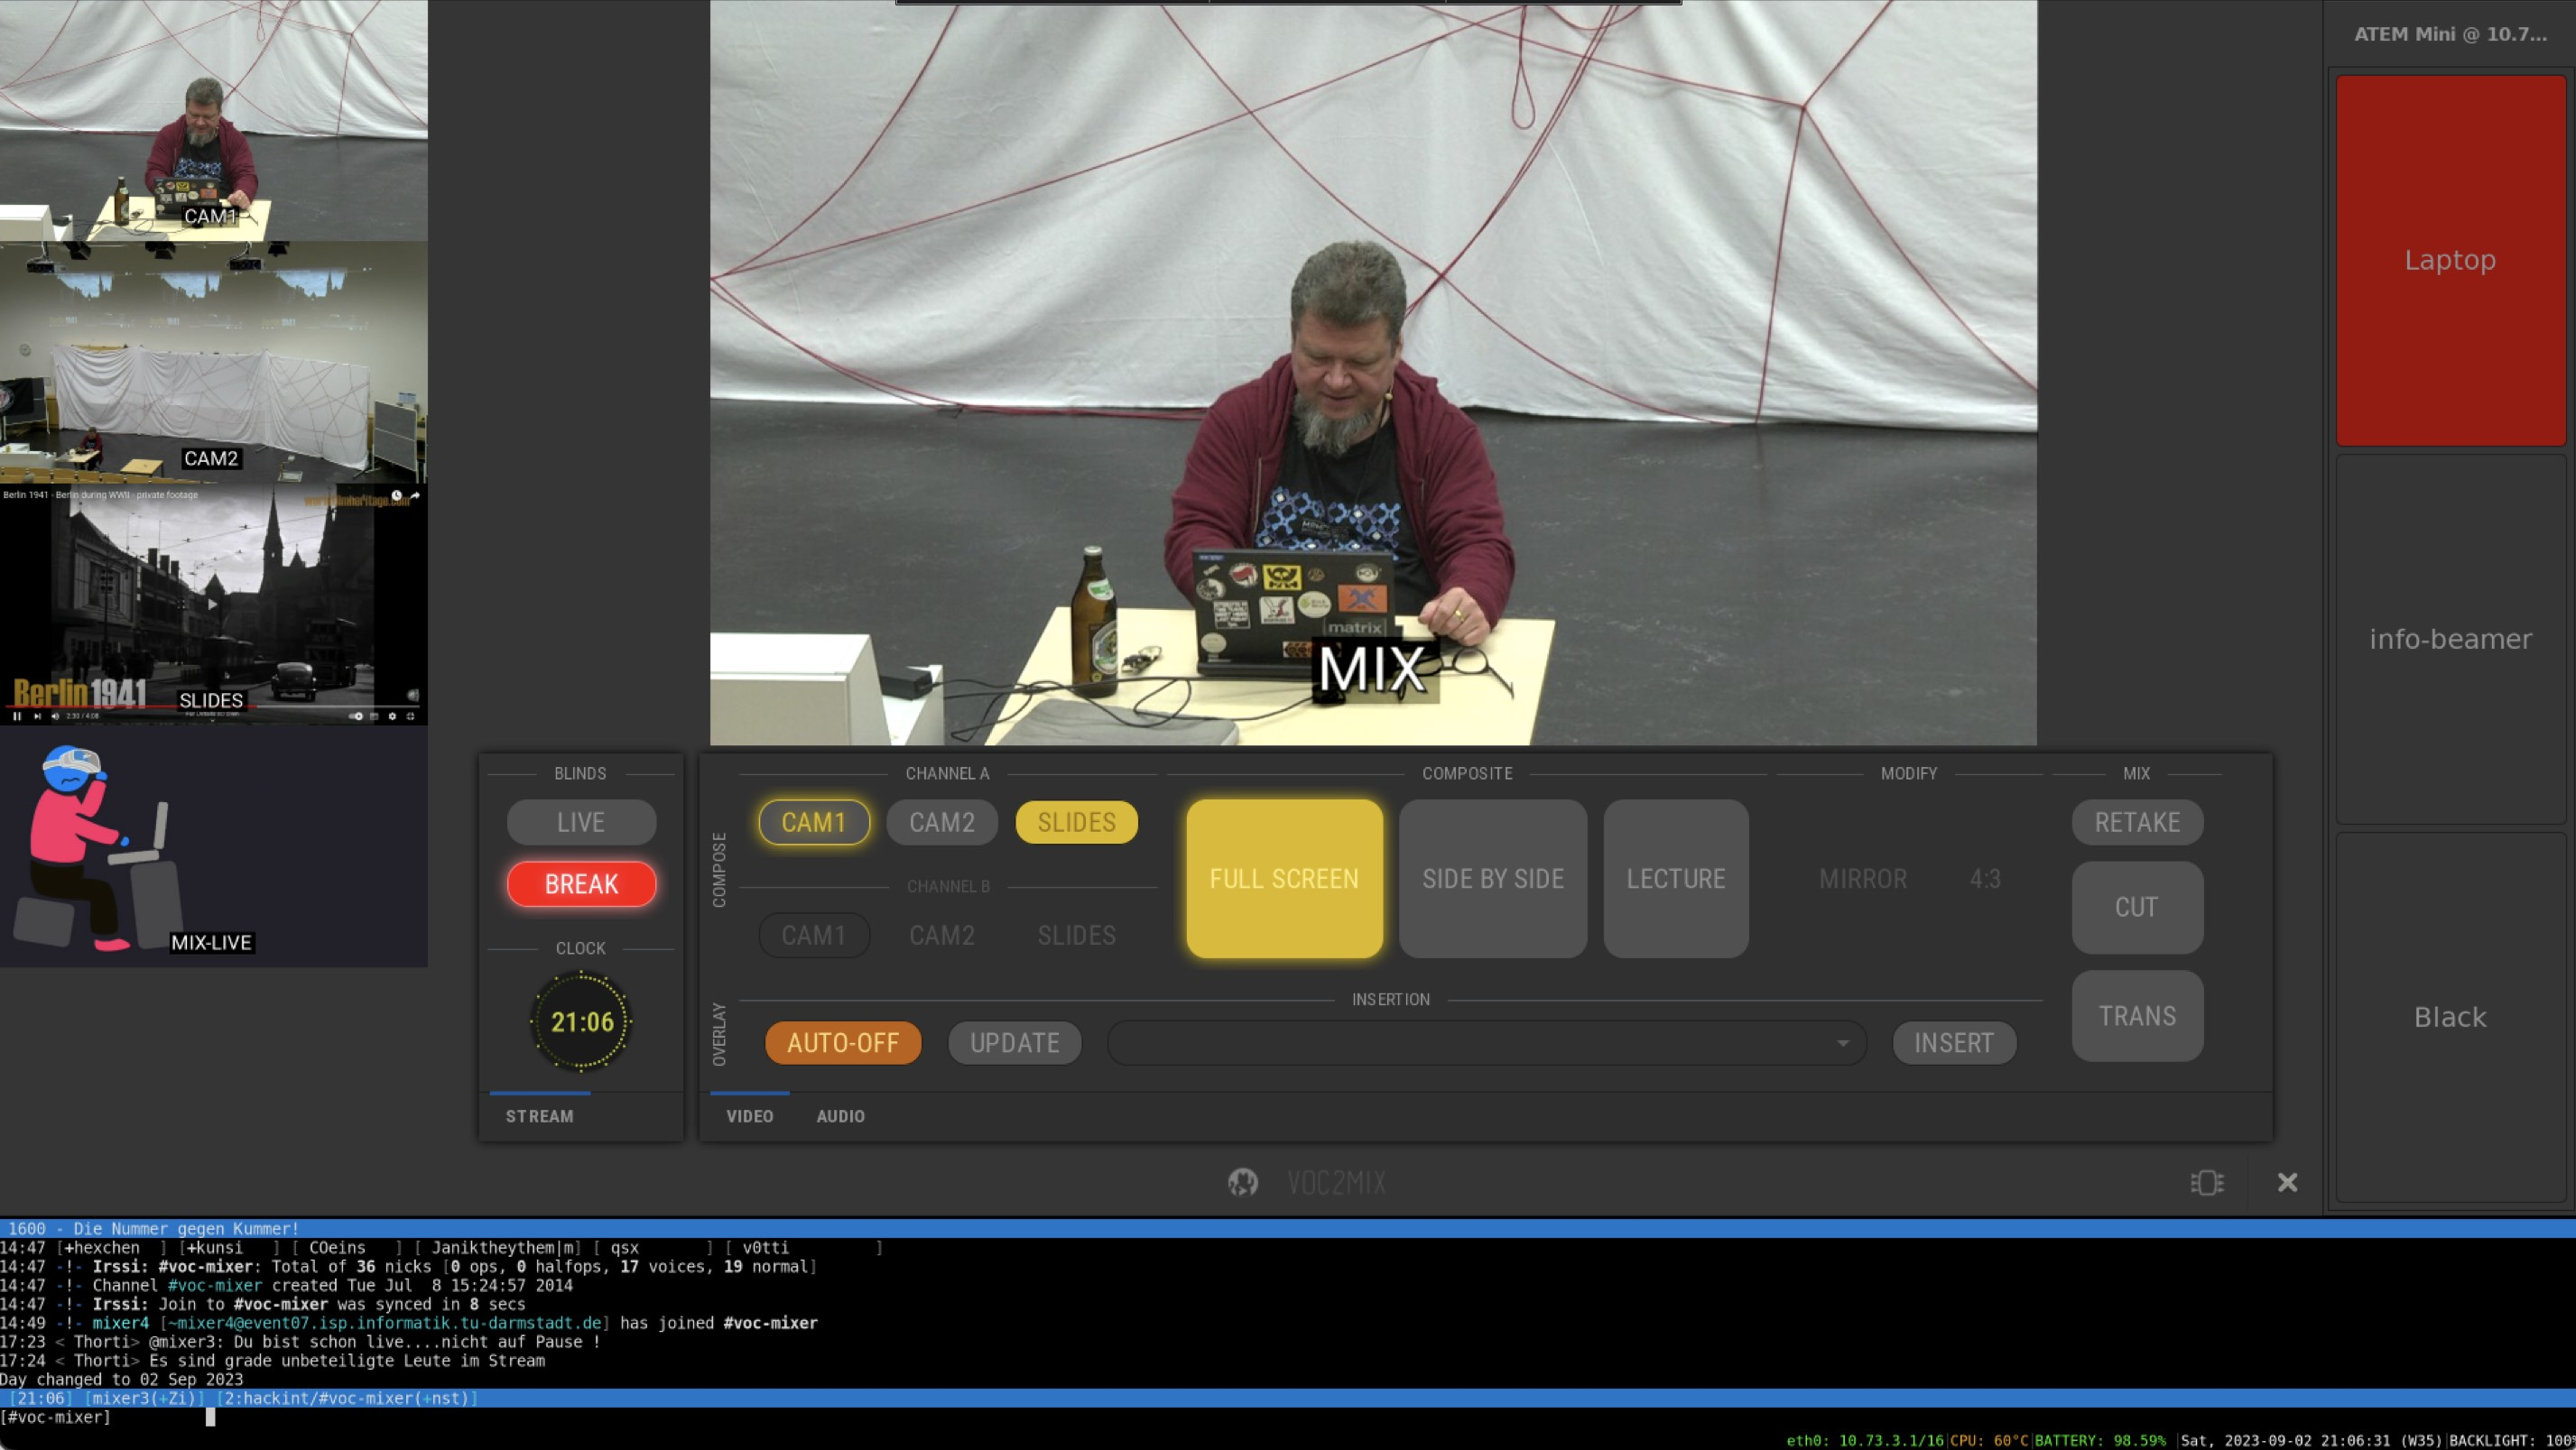
\includegraphics[width=.8\textwidth]{images/voctomix2-overview.jpg}
		% To say: Voctomix in the middle, py-atem-gtk, mix live/pause, IRC
		\caption{Voctomix2 - Overview}
	\end{figure}
\end{frame}

\begin{frame}{Voctomix2 - Pre-Select}
	\begin{figure} 
		\centering
		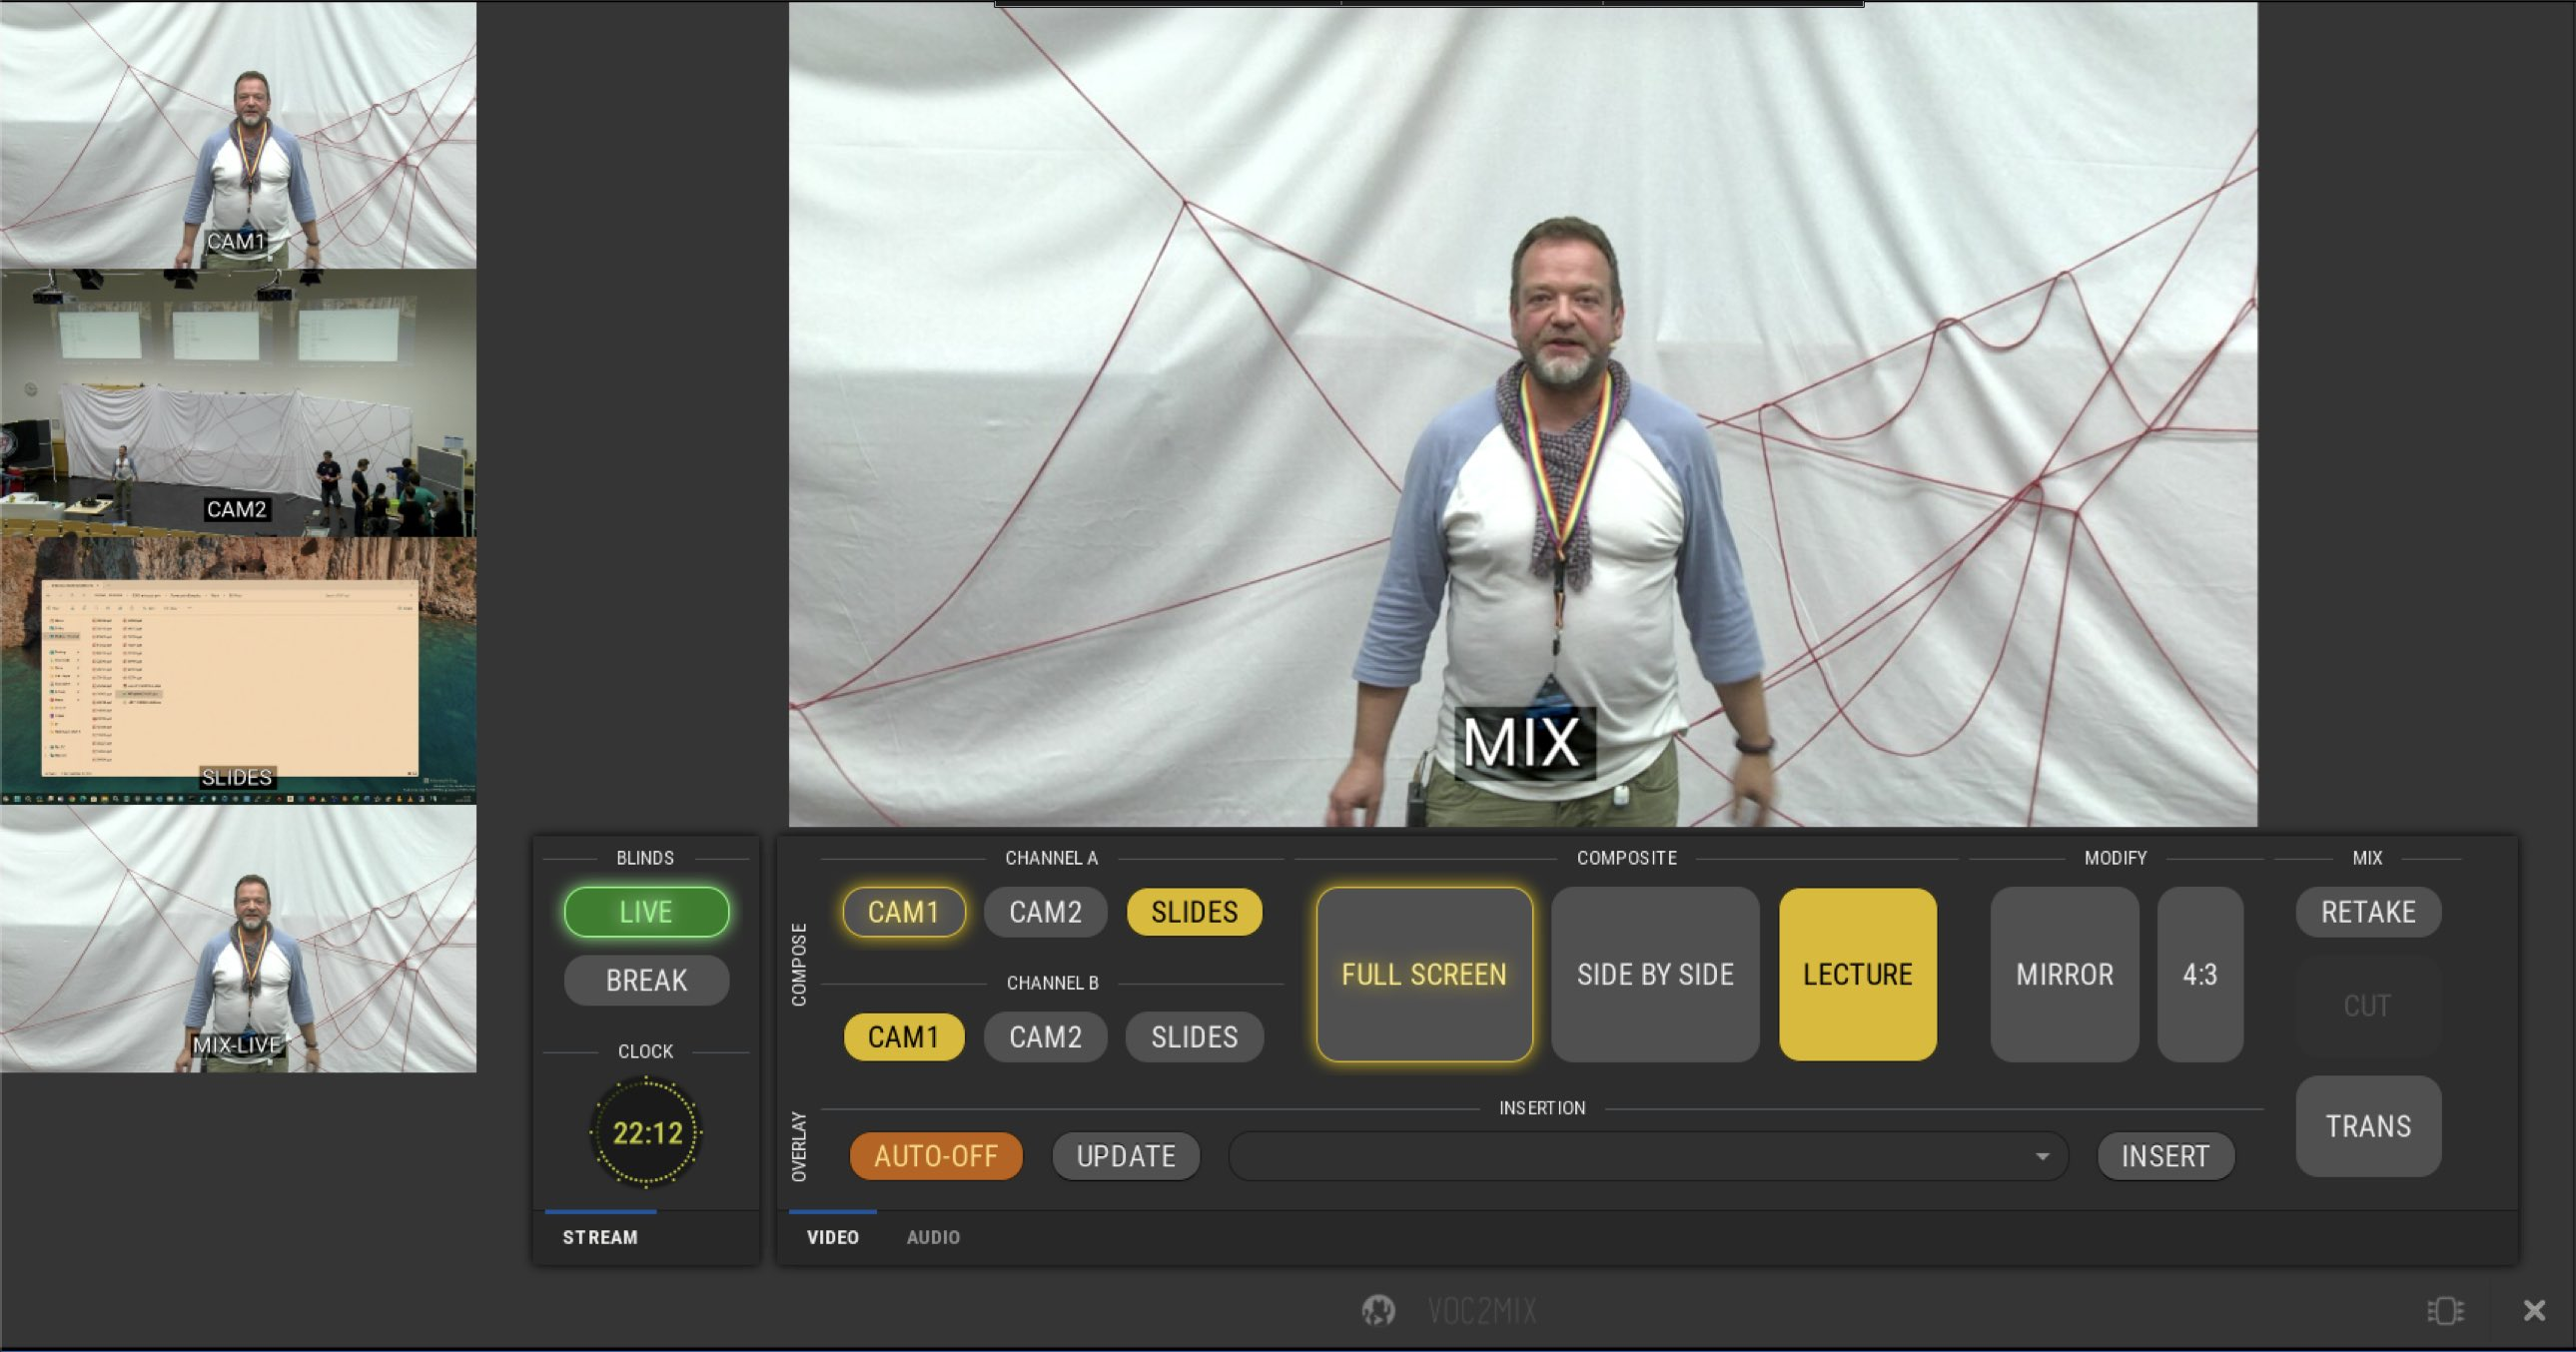
\includegraphics[width=.9\textwidth]{images/voctomix2-lecture_select.jpg}
		% To say: Next scene is shown with solid color, current scene with border, switch with trans or cut button
		\caption{Voctomix2 - Select (Lecture Mode)}
	\end{figure}
\end{frame}

\begin{frame}{Voctomix2 - Lecture Mode}
	\begin{figure} 
		\centering
		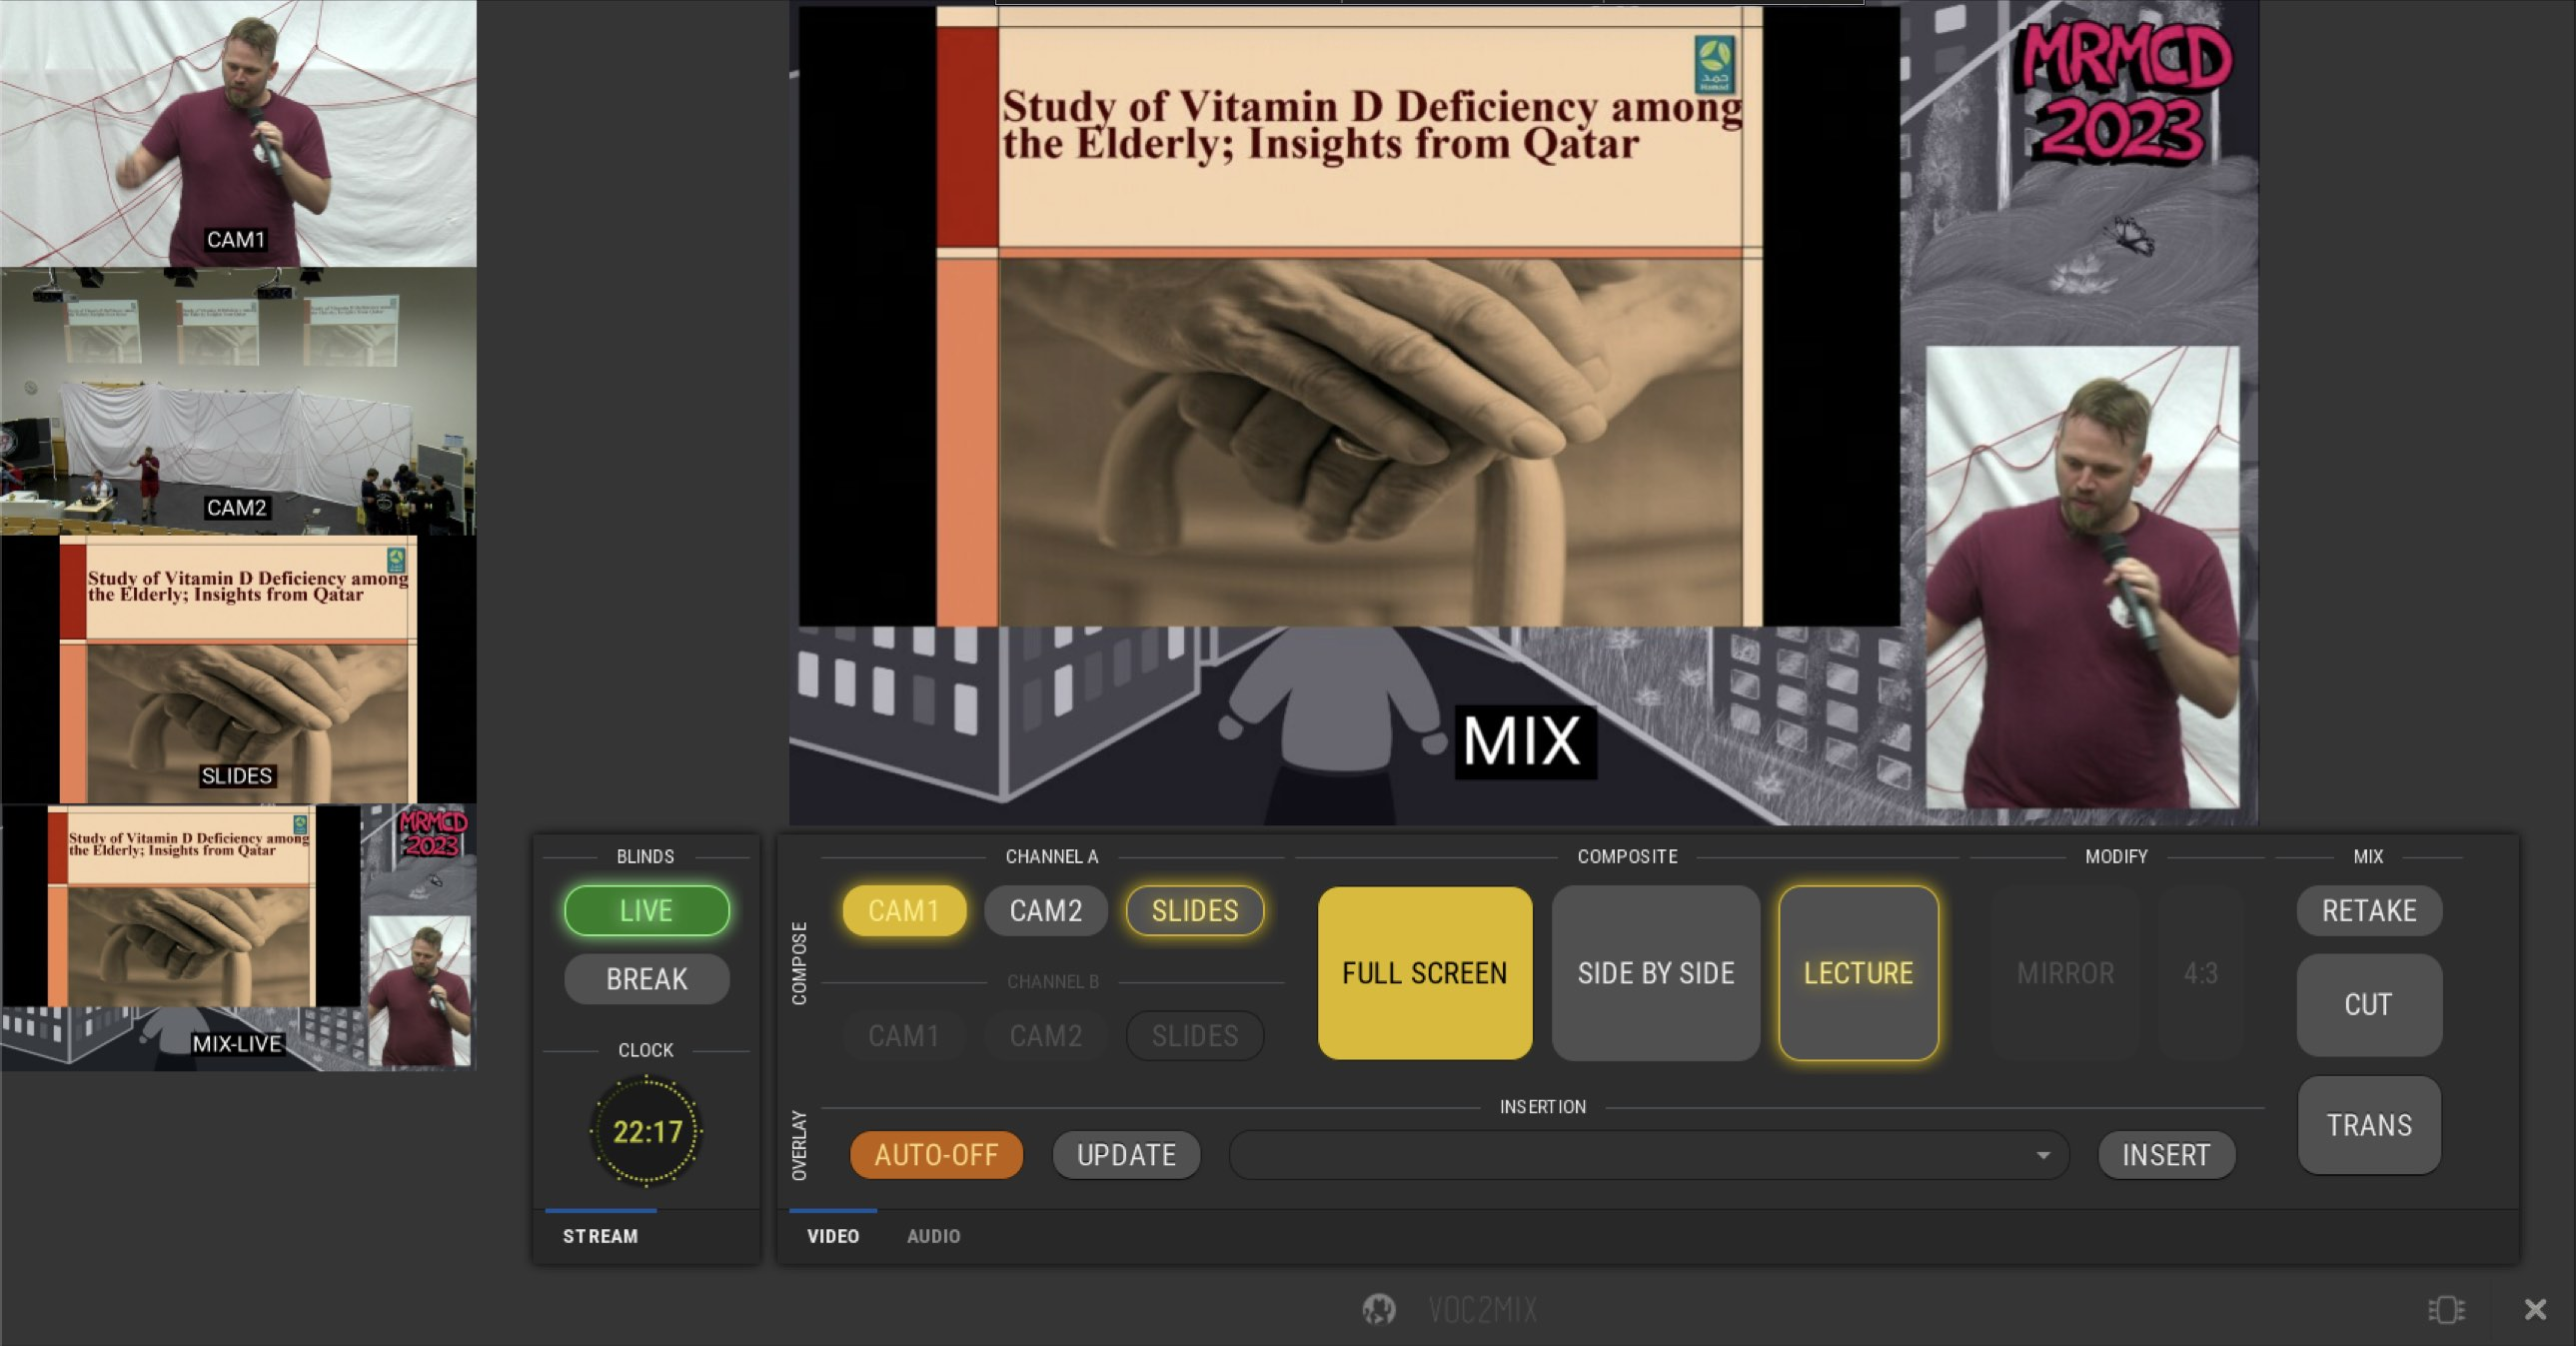
\includegraphics[width=.9\textwidth]{images/voctomix2-lecture.jpg}
		% To say: Pre-select and live mix switch places
		\caption{Voctomix2 - Lecture Mode}
	\end{figure}
\end{frame}

\begin{frame}{Voctomix2 - Lecture Mode 4:3}
	\begin{figure} 
		\centering
		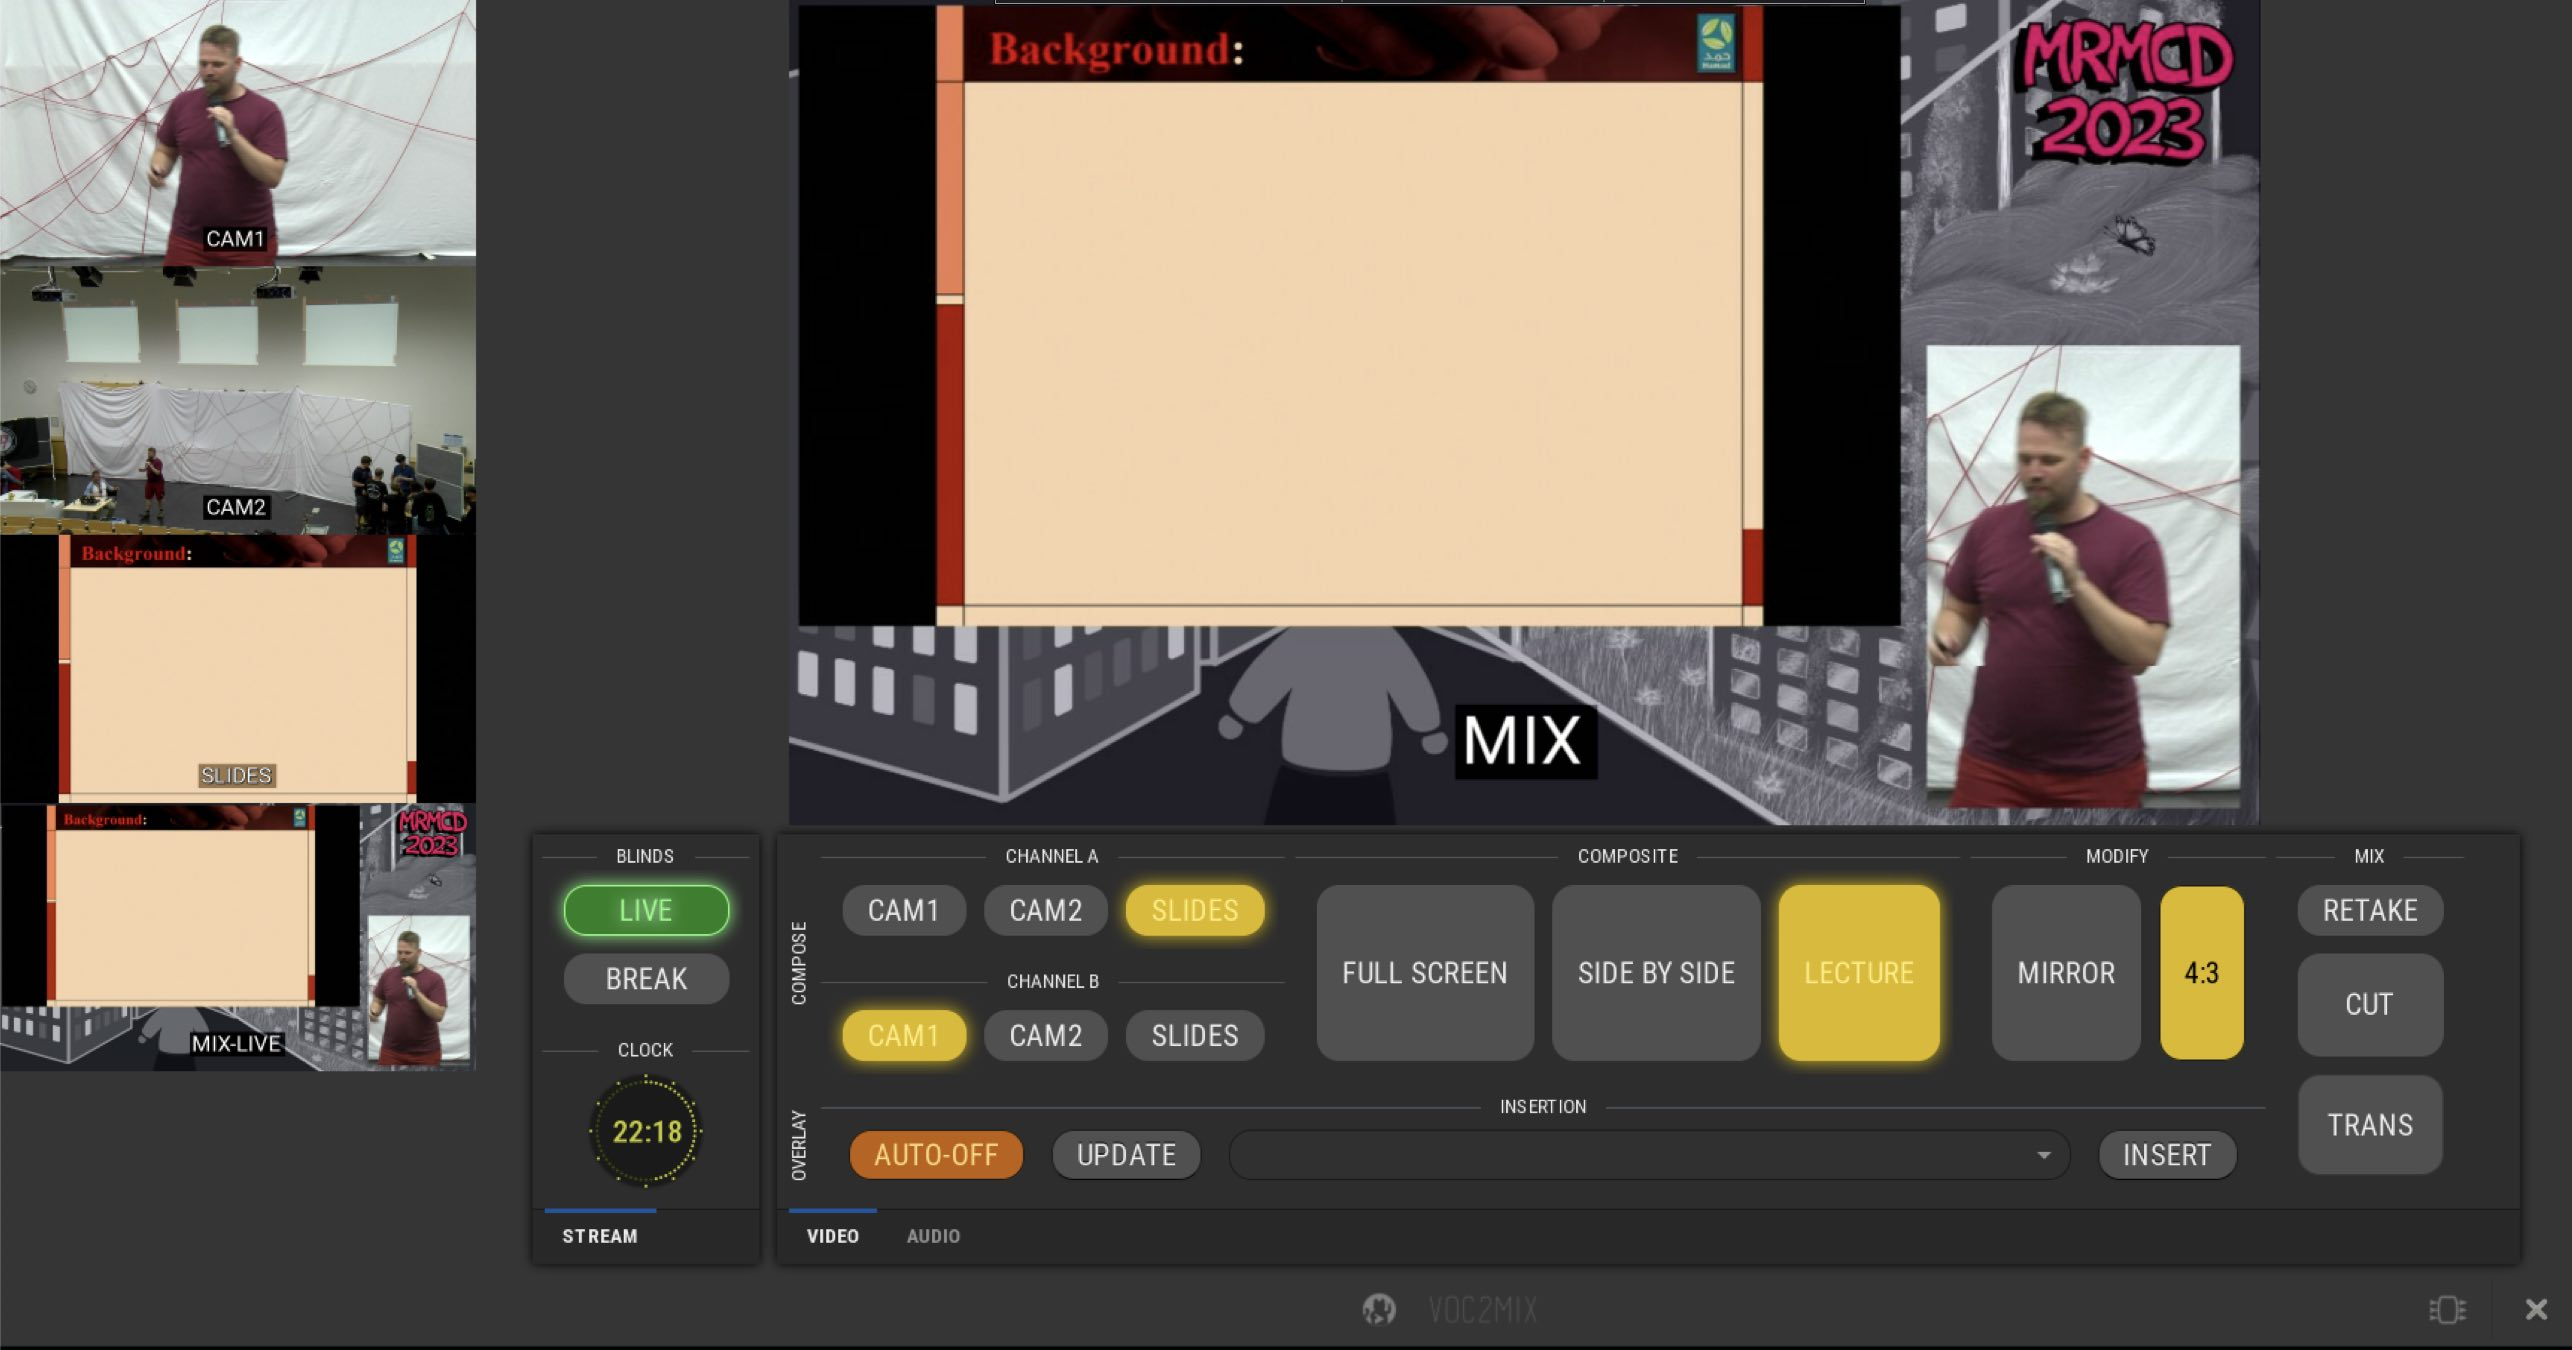
\includegraphics[width=.9\textwidth]{images/voctomix2-lecture_43_select.jpg}
		% To say: Select 4:3 mode
		\caption{Voctomix2 - Select Lecture Mode 4:3}
	\end{figure}
\end{frame}

\begin{frame}{Voctomix2 - Lecture Mode 4:3}
	\begin{figure} 
		\centering
		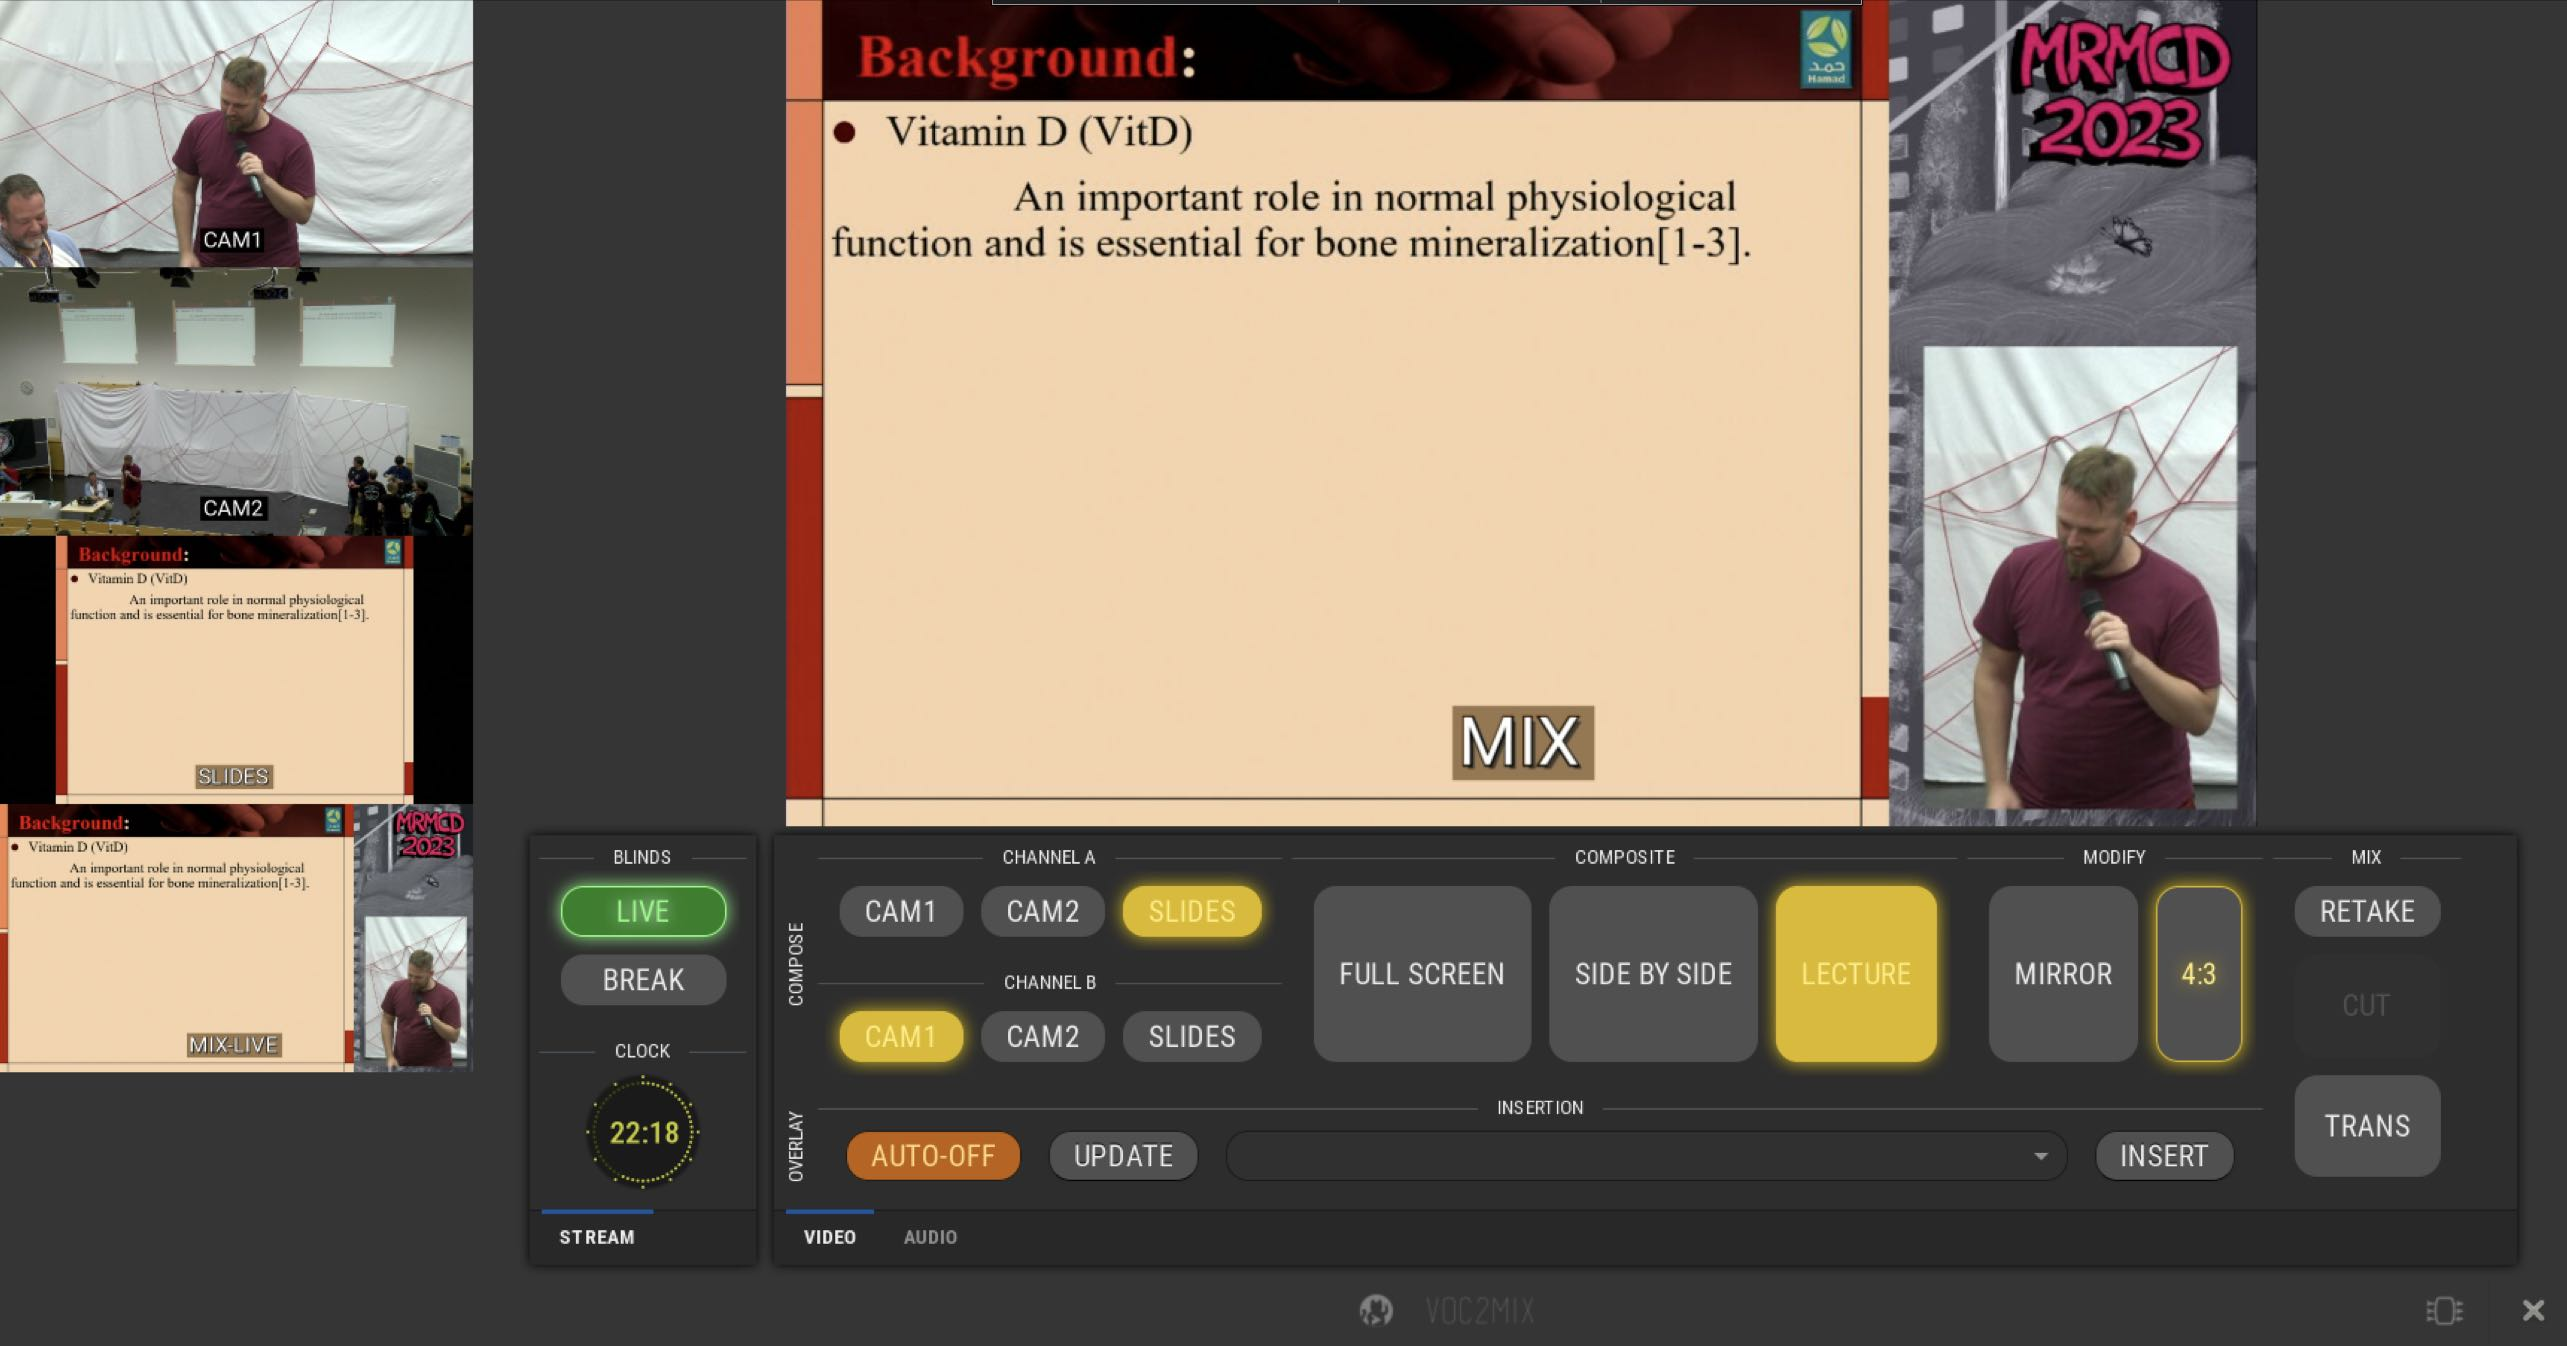
\includegraphics[width=.9\textwidth]{images/voctomix2-lecture_43.jpg}
		% To say: That's how 4:3 looks
		\caption{Voctomix2 - Lecture Mode 4:3}
	\end{figure}
\end{frame}

\section{Video Mixing Guidelines}
\begin{frame}{Mixing Guidelines - Hard Rules}
	\begin{itemize}
		\item \textbf{All} you are doing is \textbf{recorded} and will be published. \alert{\textbf{Don't make mistakes.}}
		\item The Audience is \textbf{not to be filmed}. Cut away if faces of people not on the stage appear.
		\item \textbf{Slides are important}
		\item Slides stay on till the text has been read \textbf{twice}.
		\item Show new slides \textbf{immediately}.
	\end{itemize}
\end{frame}

\begin{frame}{Mixing Guidelines - Softer Hints}
	\begin{itemize}
		\item Start early – opening announcements of the Herald are a good start. Their introduction has to be in the recording and on stream.
		\item Open wide – Structure the beginning of a talk with shots that set the stage
		\item The slides in fullscreen – you’re dealing with a very small screen. Text has to be readable
		\item Show gestures – medium-close-up that follows the speakers eye-line
		\item Don’t be too cutty – Pace your videos temperately. Do not cut too often.
		\item Don't end too early – All questions and answers have to be recorded. The herald ends the talk, not the mixer angel.
	\end{itemize}
	\begin{exampleblock}{Hints}
		Leave lots of room at the start and end of a talk. 
		Cut away from the infobeamer before the Herald starts with announcements. 
		Cut to the infobeamer only after the last applause has finished.
	\end{exampleblock}
\end{frame}
